% Options for packages loaded elsewhere
\PassOptionsToPackage{unicode}{hyperref}
\PassOptionsToPackage{hyphens}{url}
%
\documentclass[
]{book}
\usepackage{amsmath,amssymb}
\usepackage{iftex}
\ifPDFTeX
  \usepackage[T1]{fontenc}
  \usepackage[utf8]{inputenc}
  \usepackage{textcomp} % provide euro and other symbols
\else % if luatex or xetex
  \usepackage{unicode-math} % this also loads fontspec
  \defaultfontfeatures{Scale=MatchLowercase}
  \defaultfontfeatures[\rmfamily]{Ligatures=TeX,Scale=1}
\fi
\usepackage{lmodern}
\ifPDFTeX\else
  % xetex/luatex font selection
\fi
% Use upquote if available, for straight quotes in verbatim environments
\IfFileExists{upquote.sty}{\usepackage{upquote}}{}
\IfFileExists{microtype.sty}{% use microtype if available
  \usepackage[]{microtype}
  \UseMicrotypeSet[protrusion]{basicmath} % disable protrusion for tt fonts
}{}
\makeatletter
\@ifundefined{KOMAClassName}{% if non-KOMA class
  \IfFileExists{parskip.sty}{%
    \usepackage{parskip}
  }{% else
    \setlength{\parindent}{0pt}
    \setlength{\parskip}{6pt plus 2pt minus 1pt}}
}{% if KOMA class
  \KOMAoptions{parskip=half}}
\makeatother
\usepackage{xcolor}
\usepackage{longtable,booktabs,array}
\usepackage{calc} % for calculating minipage widths
% Correct order of tables after \paragraph or \subparagraph
\usepackage{etoolbox}
\makeatletter
\patchcmd\longtable{\par}{\if@noskipsec\mbox{}\fi\par}{}{}
\makeatother
% Allow footnotes in longtable head/foot
\IfFileExists{footnotehyper.sty}{\usepackage{footnotehyper}}{\usepackage{footnote}}
\makesavenoteenv{longtable}
\usepackage{graphicx}
\makeatletter
\def\maxwidth{\ifdim\Gin@nat@width>\linewidth\linewidth\else\Gin@nat@width\fi}
\def\maxheight{\ifdim\Gin@nat@height>\textheight\textheight\else\Gin@nat@height\fi}
\makeatother
% Scale images if necessary, so that they will not overflow the page
% margins by default, and it is still possible to overwrite the defaults
% using explicit options in \includegraphics[width, height, ...]{}
\setkeys{Gin}{width=\maxwidth,height=\maxheight,keepaspectratio}
% Set default figure placement to htbp
\makeatletter
\def\fps@figure{htbp}
\makeatother
\setlength{\emergencystretch}{3em} % prevent overfull lines
\providecommand{\tightlist}{%
  \setlength{\itemsep}{0pt}\setlength{\parskip}{0pt}}
\setcounter{secnumdepth}{5}
\usepackage{booktabs}
\ifLuaTeX
  \usepackage{selnolig}  % disable illegal ligatures
\fi
\usepackage[]{natbib}
\bibliographystyle{plainnat}
\IfFileExists{bookmark.sty}{\usepackage{bookmark}}{\usepackage{hyperref}}
\IfFileExists{xurl.sty}{\usepackage{xurl}}{} % add URL line breaks if available
\urlstyle{same}
\hypersetup{
  pdftitle={AI Declassified: A Ross Faculty Survival Guide},
  pdfauthor={Adam Zhang, Ryan Berger, Michelle Xu, Fuad Chedid, Sona Coshal},
  hidelinks,
  pdfcreator={LaTeX via pandoc}}

\title{AI Declassified: A Ross Faculty Survival Guide}
\author{Adam Zhang, Ryan Berger, Michelle Xu, Fuad Chedid, Sona Coshal}
\date{2023-08-06}

\begin{document}
\maketitle

{
\setcounter{tocdepth}{1}
\tableofcontents
}
\hypertarget{introduction}{%
\chapter{Introduction}\label{introduction}}

This book is intended to be a comprehensive look at the challenges faced by Ross faculty regarding the advent of Generative AI in academia. The content of this book is based on real world problems, solutions, and ideas captured from research and interviews with Ross Faculty members who are currently contending with the challenges brought on by educating in the age of Generative AI.

\hypertarget{about-us}{%
\chapter{About Us}\label{about-us}}

\hypertarget{ryan-berger}{%
\section{Ryan Berger}\label{ryan-berger}}

Hey! I'm Ryan Berger. I am a current Master's of Business Analytics student at Michigan Ross. In my undergrad, I also attended Michigan through the School of Information, studying data analytics. I am from New Jersey, which means I am a Giants fan and I like to say I'm from New York. Go Blue!

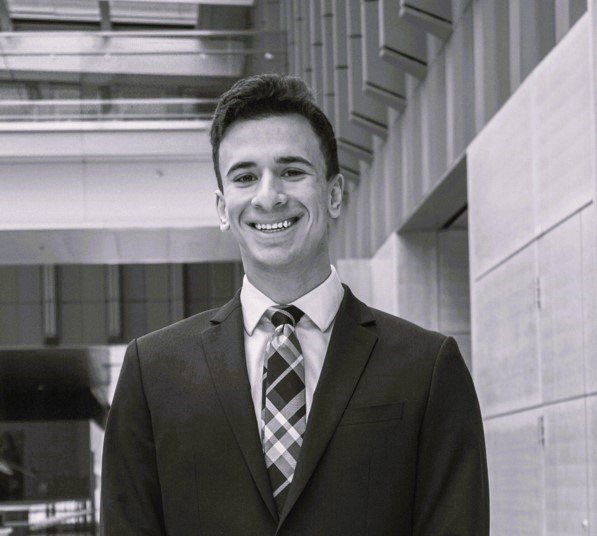
\includegraphics[width=0.4\linewidth]{rtberger}

\hypertarget{adam-zhang}{%
\section{Adam Zhang}\label{adam-zhang}}

Hi! I'm Adam Zhang. I am a Master of Business Analytics student at the Ross School of Business at University of Michigan. I attended University of Illinois Urbana-Champaign where I majored economics for undergrad. I enjoy cooking, watching movies, listening to musics (mainly 70s and 80s), and going to art museums.

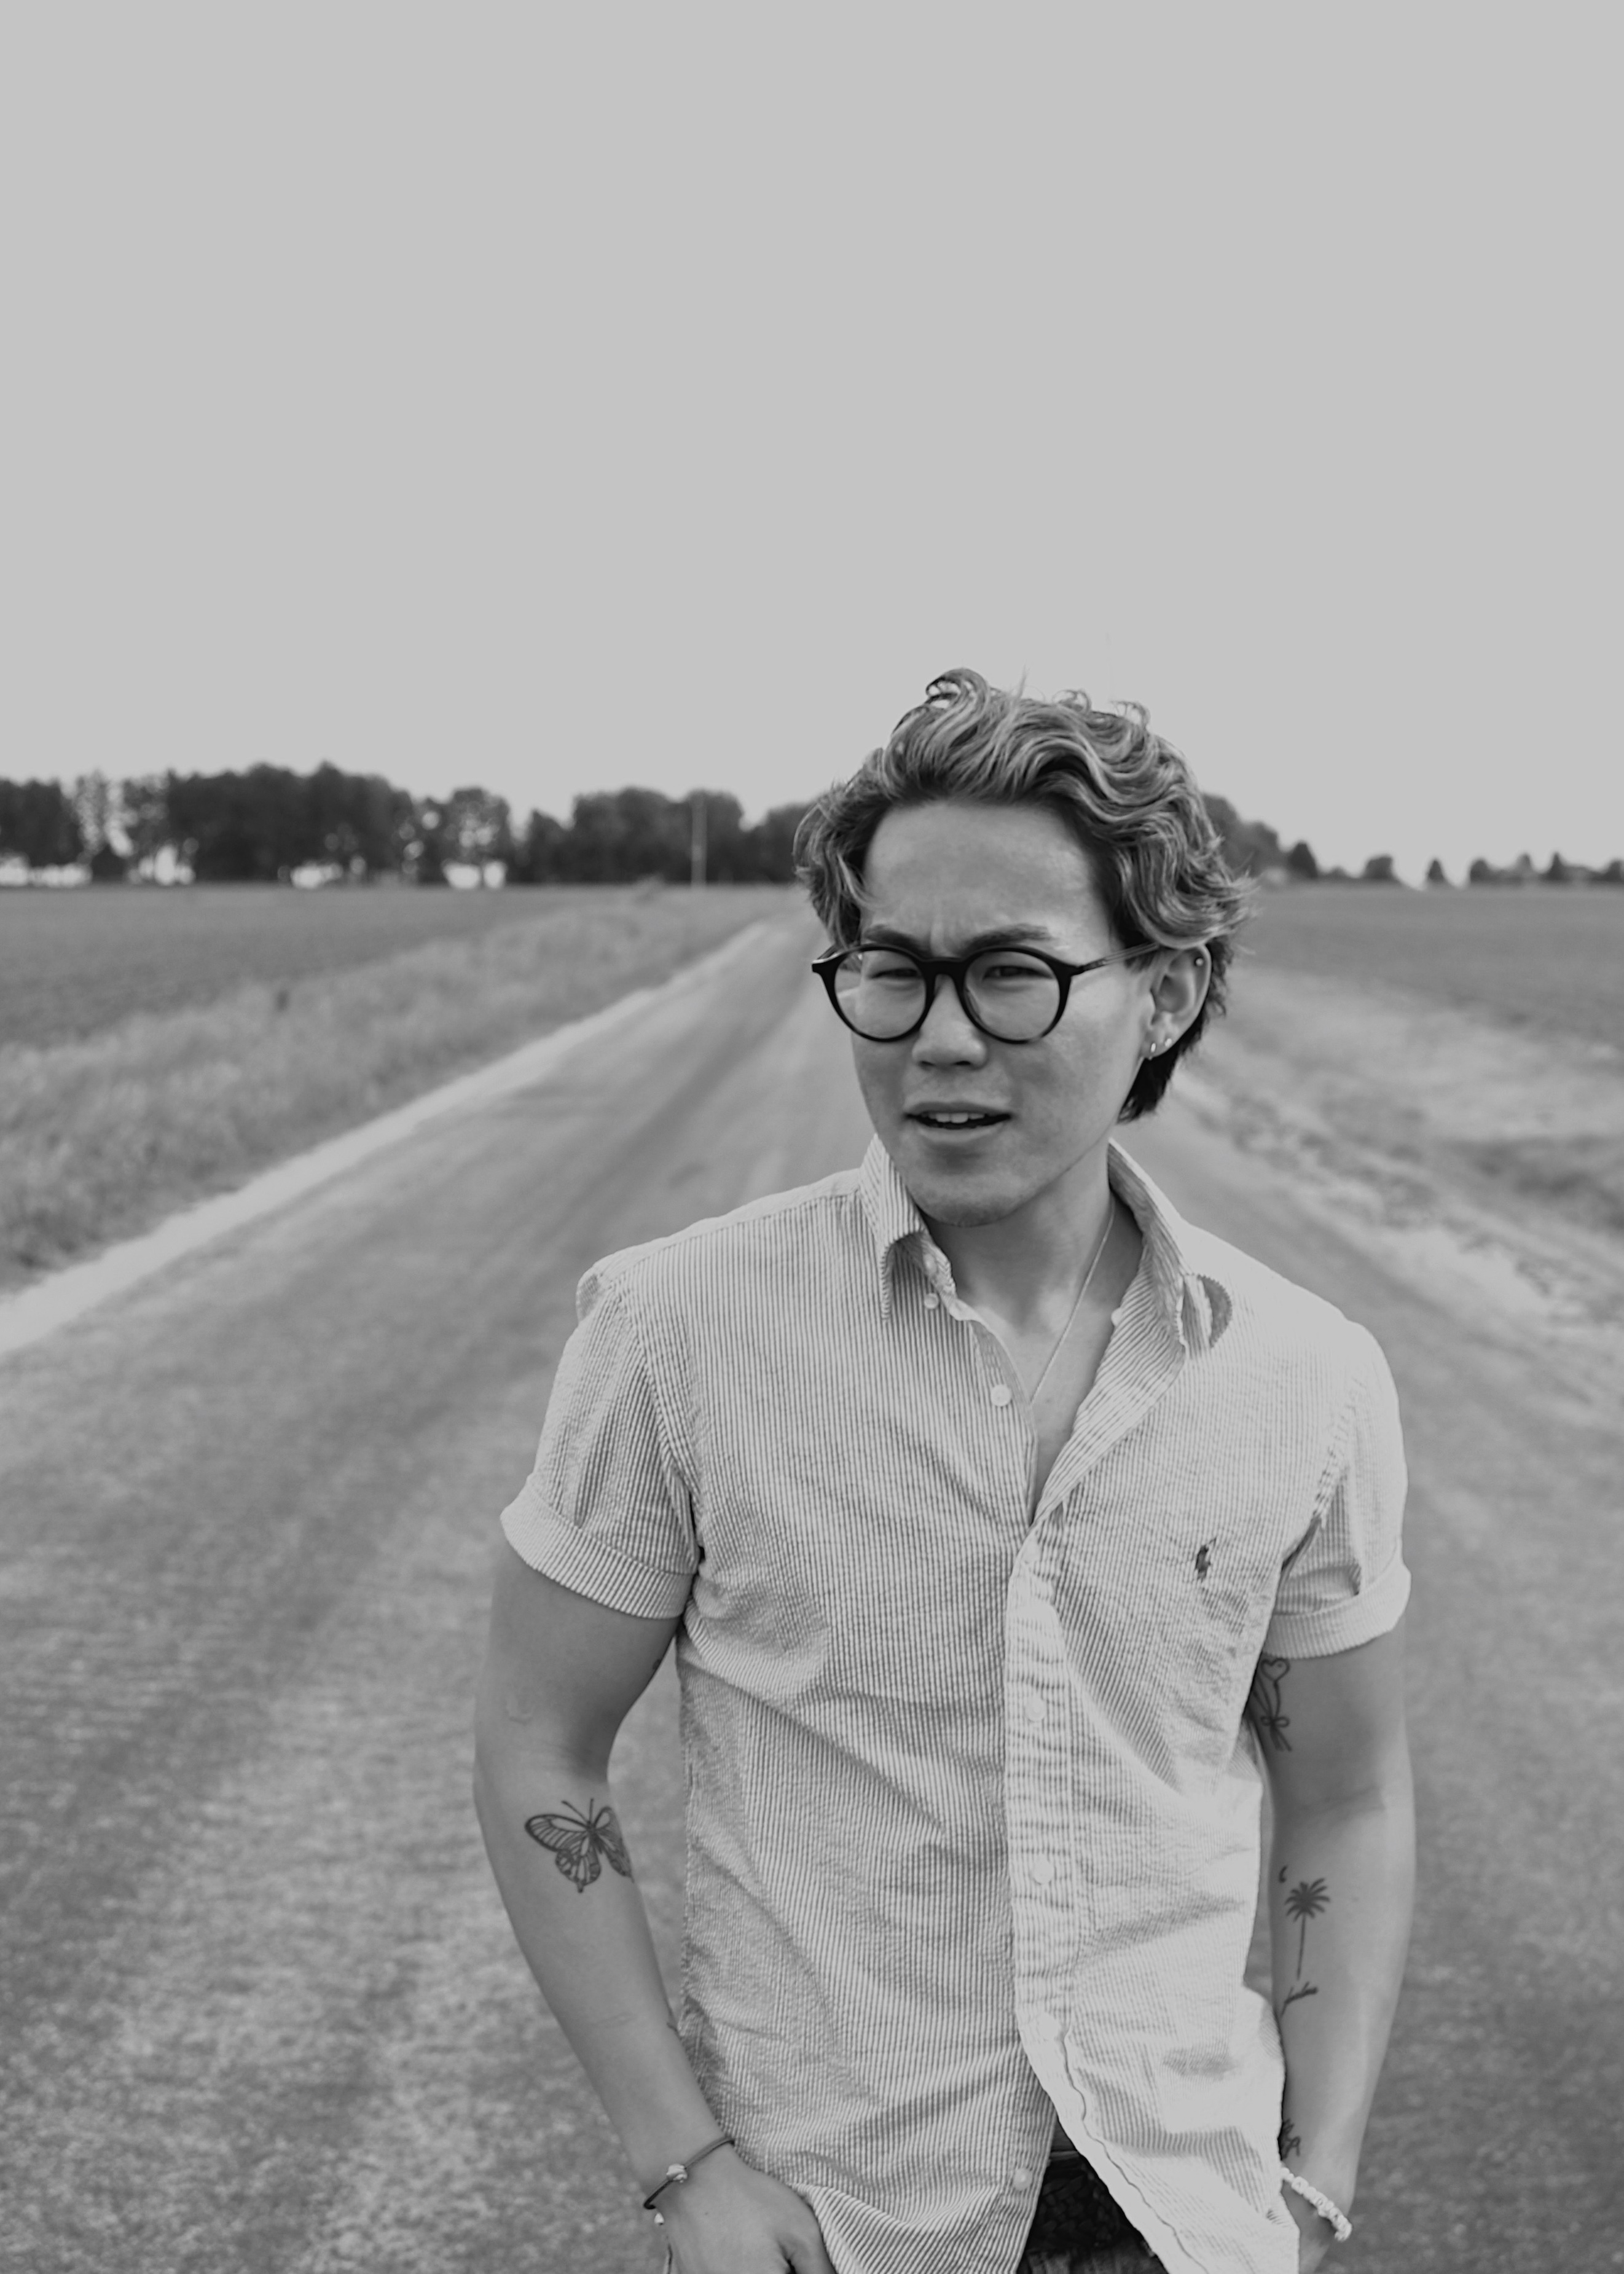
\includegraphics[width=0.4\linewidth]{AZ}

\hypertarget{michelle-xu}{%
\section{Michelle Xu}\label{michelle-xu}}

Hello, I'm Michelle Xu, originally from China. I spent six years living in the beautiful city of San Diego, California. After high school, I moved to Ann Arbor, Michigan, to pursue a major in Bioinformatics at LS\&A. Currently, I'm a Master of Business Analytics student at the University of Michigan, Ross School of Business.

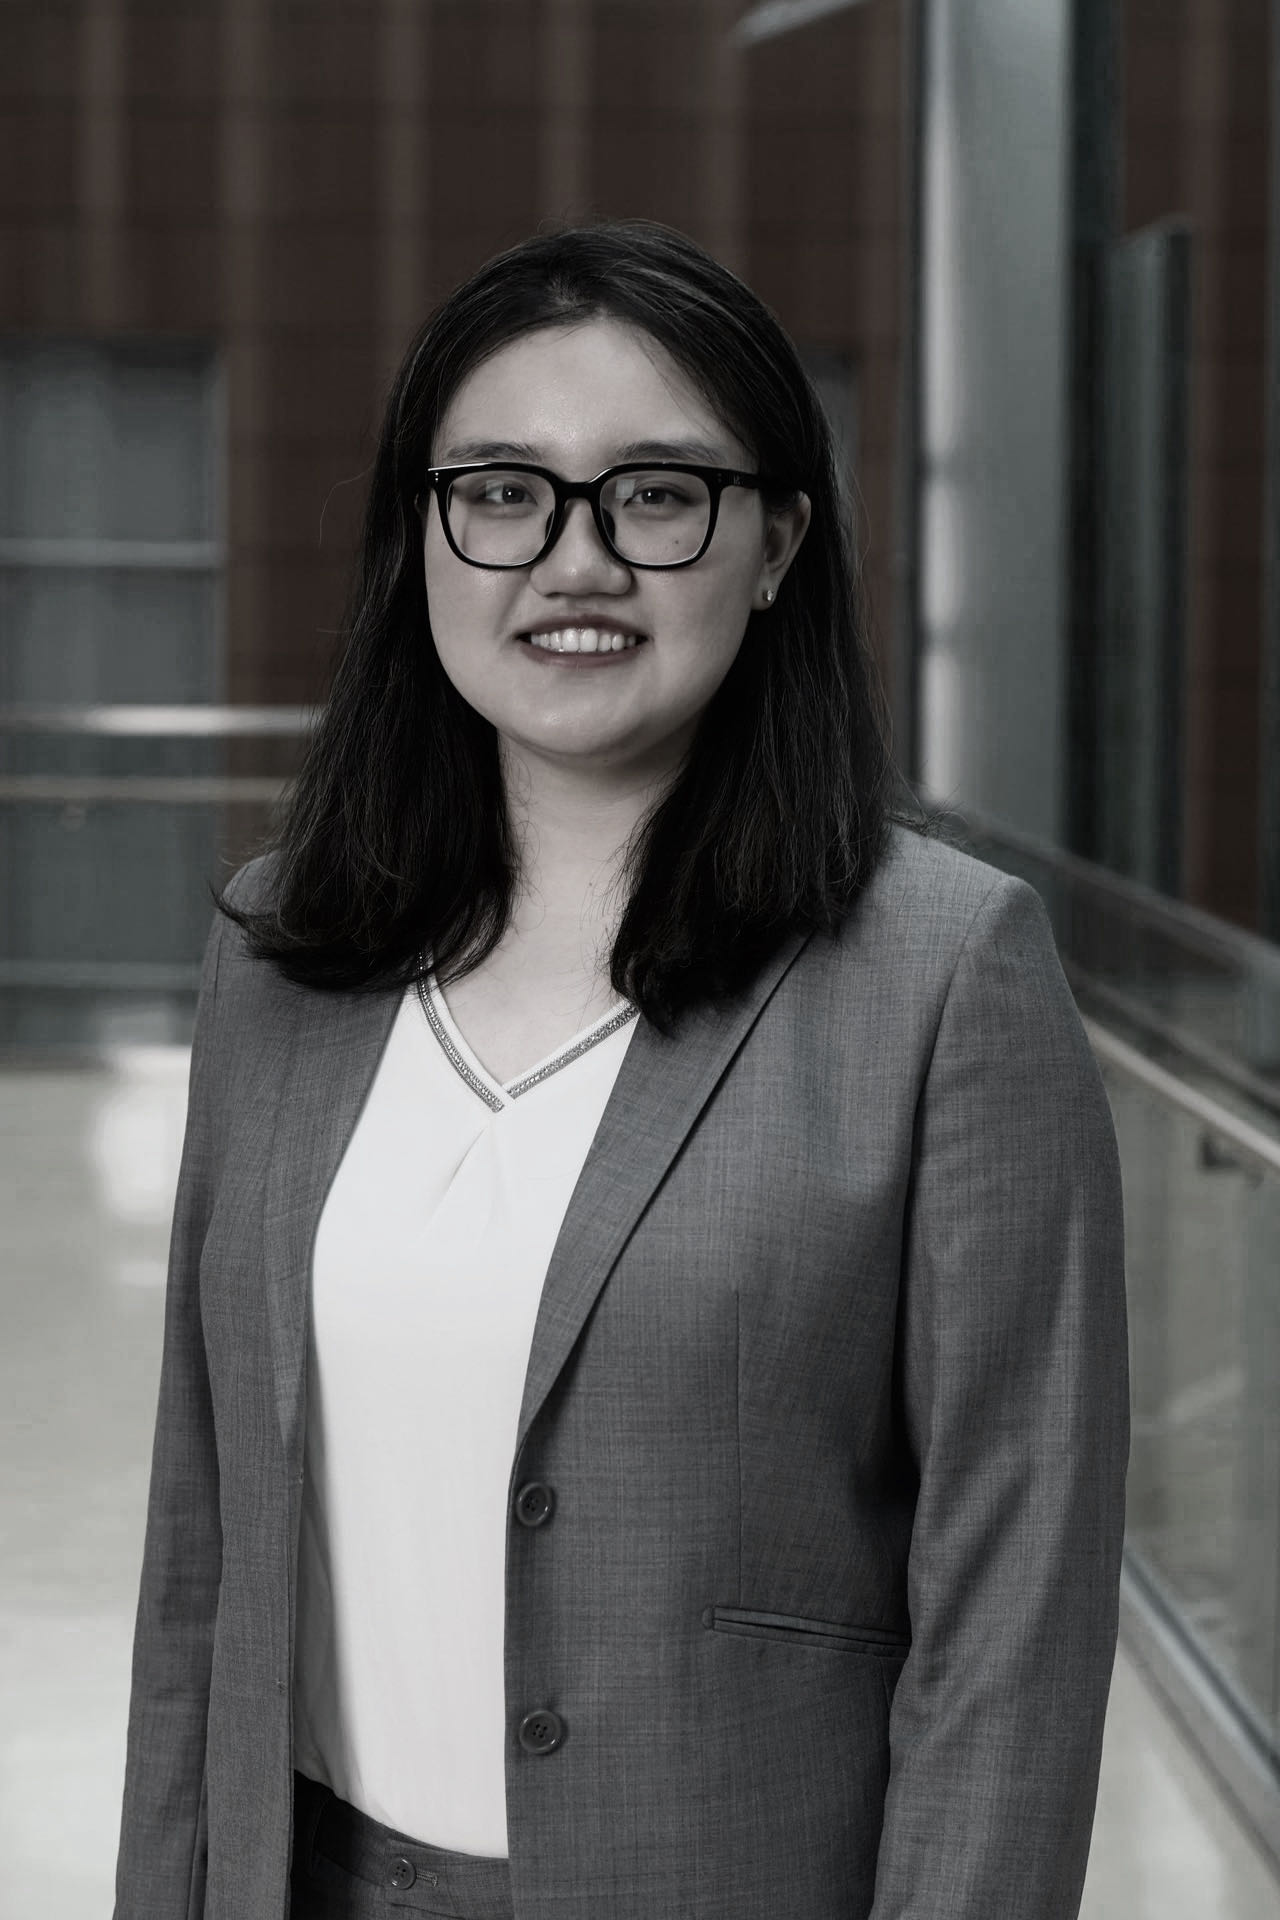
\includegraphics[width=0.4\linewidth]{WechatIMG10}

\hypertarget{sona-coshal}{%
\section{Sona Coshal}\label{sona-coshal}}

Hi, my name is Sona! I'm born and raised in Columbia, South Carolina and a proud USC Gamecock! I have a BSBA in Finance and Supply Chain from the Darla Moore School Business.

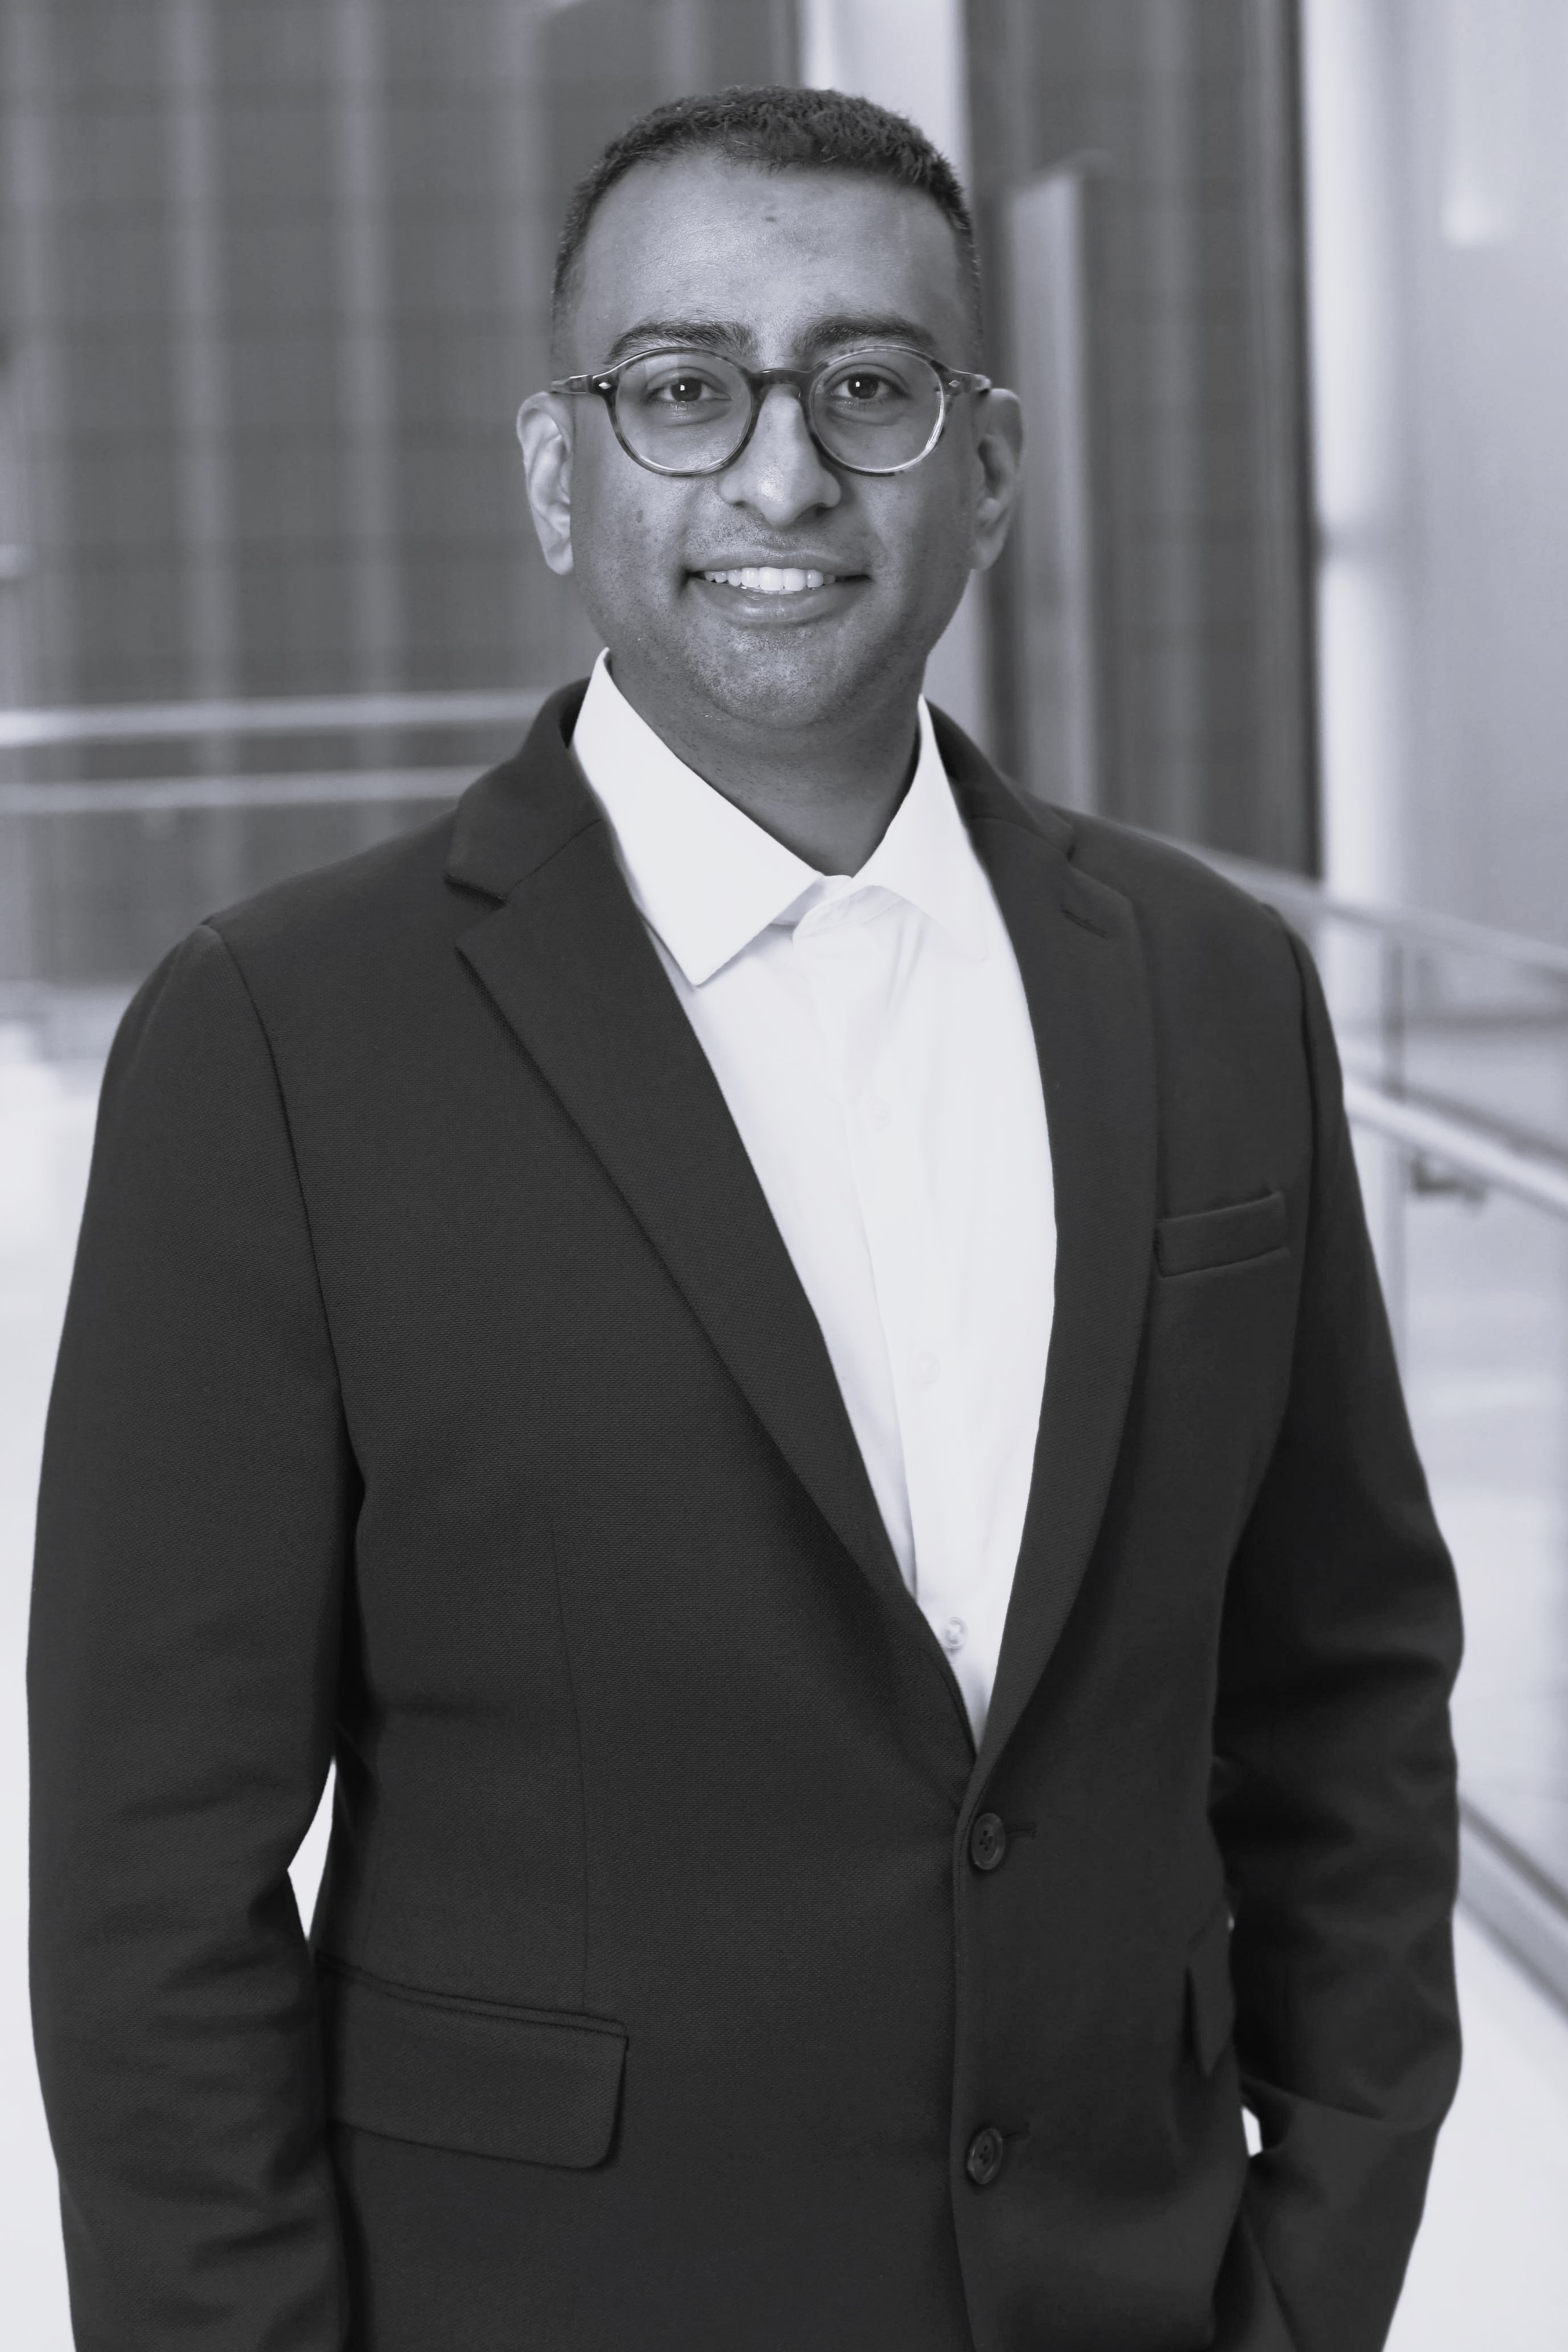
\includegraphics[width=0.4\linewidth]{Sona's_Photo}

\hypertarget{fuad-chedid}{%
\section{Fuad Chedid}\label{fuad-chedid}}

Hi! I'm Fuad, a native Michigander! Before joining the Master of Business Analytics program at Michigan Ross, I was based in Dubai, UAE. I consider myself a ``tech head'' and my main area of interest is the intersection of business and technology. I enjoy travelling and so far have visited 27 countries and five continents.

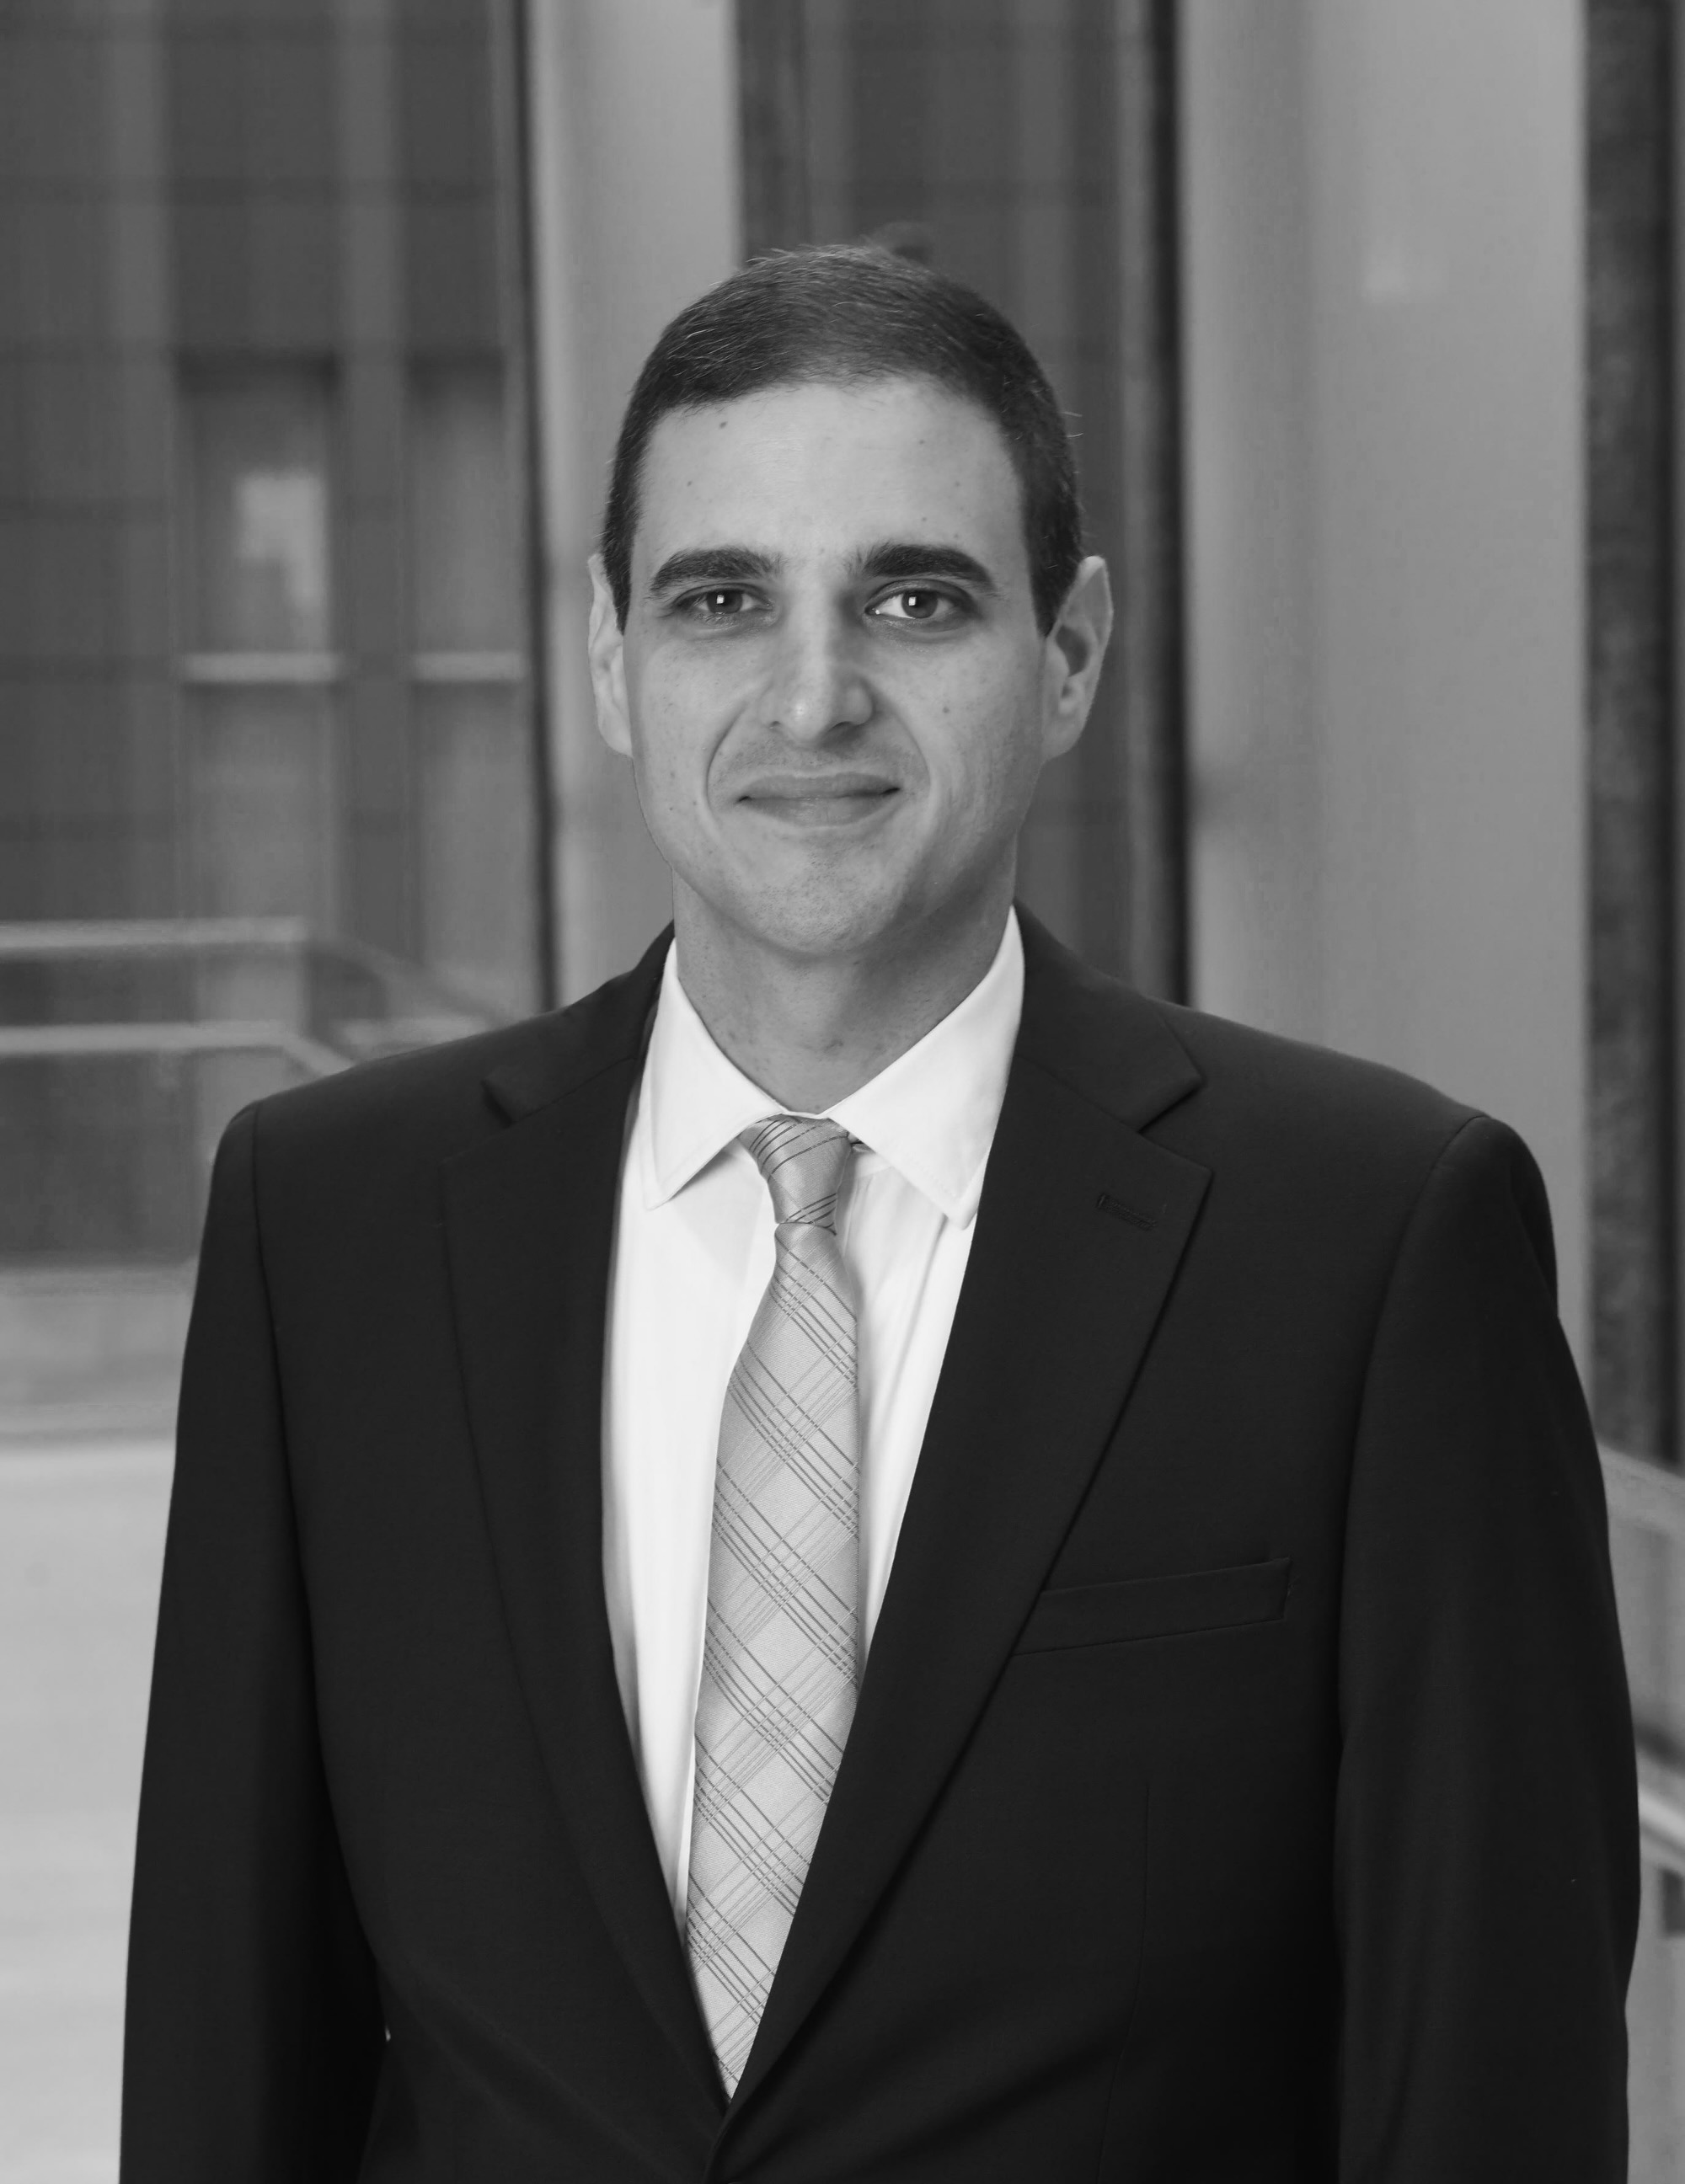
\includegraphics[width=0.4\linewidth]{fpic}

\hypertarget{current-state-of-affairs}{%
\chapter{Current State of Affairs}\label{current-state-of-affairs}}

Since the proliferation of publicly available generative AI in November 2022, U-M has been positioning itself to respond and adapt. Undoubtedly, there is a need for institutional understanding and action to ensure that generative AI is leveraged in support of the University's mission. This section provides information on the currently published university-wide guidance.

\hypertarget{u-m-genai-website}{%
\section{U-M GenAI Website}\label{u-m-genai-website}}

Recently established by the GAIA Committee (see \ref{gaia-committee}), \url{https://genAI.umich.edu} is a comprehensive resource containing the latest guidance and information for all members of the U-M community.

\hypertarget{gaia-committee}{%
\section{GAIA Committee}\label{gaia-committee}}

The Generative AI Advisory (\href{https://it.umich.edu/strategy-planning/gaia}{GAIA}) Committee was established in the first half of 2023, with the overall aim being:

\begin{quote}
to provide guidance to the university community for the use of generative AI and provide strategic advice to the~VPIT-CIO~and Provost.
\end{quote}

An overview of the committee's \href{https://genai.umich.edu/committee-report}{official report}, published on June 30th 2023, is provided in section \ref{initial-report-june-30-2023}.

The committee includes members from the following schools, colleges, and departments:

\begin{longtable}[]{@{}ll@{}}
\caption{\emph{As of Aug 2023. Note: Some members represent more than one affiliation.}}\tabularnewline
\toprule\noalign{}
School / College / Department & \# of Member(s) \\
\midrule\noalign{}
\endfirsthead
\toprule\noalign{}
School / College / Department & \# of Member(s) \\
\midrule\noalign{}
\endhead
\bottomrule\noalign{}
\endlastfoot
\textbf{Executive Sponsor} & 1 \\
\textbf{College of Engineering} & 4 \\
\textbf{Medical School} & 2 \\
\textbf{School of Public Health} & 1 \\
\textbf{College of Literature, Science, and the Arts} & 3 \\
\textbf{School of Education} & 2 \\
\textbf{School of Information} & 2 \\
\textbf{Ross School of Business} & 2 \\
\textbf{Information and Technology Services} & 1 \\
\textbf{Center for Research on Learning and Teaching} & 1 \\
\textbf{Center for Academic Innovation} & 1 \\
\textbf{Office of the Vice Provost, DE\&I} & 1 \\
\textbf{U-M Flint} & 1 \\
\textbf{U-M Dearborn} & 1 \\
\end{longtable}

\hypertarget{initial-report-june-30-2023}{%
\subsection{Initial Report (June 30 2023)}\label{initial-report-june-30-2023}}

\hypertarget{key-benefits-and-opportunities}{%
\subsubsection*{Key Benefits and Opportunities}\label{key-benefits-and-opportunities}}
\addcontentsline{toc}{subsubsection}{Key Benefits and Opportunities}

\begin{quote}
\begin{itemize}
\item
  GenAI will enable U-M to advance its mission and accelerate and support Vision 2034.
\item
  GenAI has the potential to transform teaching outcomes by creating customizable learning pathways
\item
  GenAI will accelerate knowledge development,including rethinking of disciplinary boundaries and domains, and possibly, defining new ones.
\item
  From an efficiency perspective, GenAI has the potential to support enhanced administrative productivity and service quality throughout the University.
\item
  \textbf{U-M has the intellectual depth, resources, and international and national connections and networks to be the leader in the development and appropriate use of GenAI.}
\end{itemize}
\end{quote}

\hypertarget{key-threats-and-weaknesses}{%
\subsubsection*{Key Threats and Weaknesses}\label{key-threats-and-weaknesses}}
\addcontentsline{toc}{subsubsection}{Key Threats and Weaknesses}

\begin{quote}
\begin{itemize}
\item
  Several technical weaknesses currently exist, including temporal ignorance, hallucination and fabrication, misattribution, overriding safety protocols, inadvertent inclusion breaches or ethical problems, and bias in training data.
\item
  Social weaknesses refer to those that arise from the interaction between the system and user, which may yield unanticipated actions and outcomes. While myriad and evolving, a few examples of social weaknesses include

  \begin{itemize}
  \item
    rapid escalation of deep fakes in video and audio,
  \item
    user attribution of output generated by GenAI to themselves or others,
  \item
    GenAI companion giving dangerous advice to children,
  \item
    use of GenAI to perform research without appropriate disclosure,
  \item
    inappropriate use of prompt data by AI provider,
  \item
    reduced demand for human labor in many professions,
  \item
    inequitable access to state-of-the-art GenAI systems,
  \item
    and unauthorized generation or replication of copyrighted or otherwise protected material.
  \end{itemize}
\end{itemize}
\end{quote}

\hypertarget{overall-recommendations}{%
\subsubsection*{Overall Recommendations}\label{overall-recommendations}}
\addcontentsline{toc}{subsubsection}{Overall Recommendations}

A brief highlight of the recommendations provided in the report:

\begin{quote}
\begin{itemize}
\item
  Dissemination of guidance and launch of campus discussion (Timeline: immediate).
\item
  Teaching, Learning, and Academic Innovation (Timeline: Fall 2023). U-M can approach GenAI as an opportunity to rethink how we teach and define meaningful learning objectives, promote inclusion and equity, and assess learning. \textbf{Instructors should be given complete flexibility to allow or disallow the use of GenAI tools.}
\item
  Assess the use of GenAI in research and set best practice standards for privacy protections; data use controls; and updating research integrity reated SPGs, PEERS modules, and RCR training.
\item
  Provost, VPR and VPIT should establish a U-M wide research initiative in the area of Generative AI (Timeline: Fall 2023/Winter 2024).

  \begin{itemize}
  \tightlist
  \item
    U-M should consider developing its own version of foundation GenAI models to enable research and innovation (Timeline: Begin activities in Fall 2023).
  \end{itemize}
\item
  Expansion of IT infrastructure to accommodate secure and equitable access to GenAI plat- forms and tools (Timeline: Immediate and Variable).

  \begin{itemize}
  \tightlist
  \item
    Create and deliver new GenAI services. These services will be offered across three tiers, each catering to different needs and technical proficiencies and made available to Ann Arbor, Flint, and Dearborn.
  \end{itemize}
\item
  VPIT to work with the GAIA committee to coordinate and establish an AI digital commons where our community can share best practices and emerging ideas in GenAI (Timeline: Immediate).
\item
  Launch a U-M GenAI website providing strategy, policies, resources, and links. Coordinate this with a well-defined communication plan (Timeline: Immediate).
\end{itemize}
\end{quote}

\hypertarget{instructor-recommendations}{%
\subsubsection*{Instructor Recommendations}\label{instructor-recommendations}}
\addcontentsline{toc}{subsubsection}{Instructor Recommendations}

The committee's initial report identifies teaching and learning as the most \emph{``immediate and significant GenAI application domain''} and provides guidance to instructors to help prepare for the Fall 2023 semester. The below sections include highlights of the guidance.

Generally, the committee finds that it is presently ``nearly impossible to enforce'' banning GenAI use in coursework. And therefore, strongly recommends that instructors consider the following questions when adapting course work:

\begin{quote}
\begin{itemize}
\item
  Should GenAI be used in the course or not---and why or why not?
\item
  If GenAI is to be used, how is the use to be documented?
\item
  Should course learning objectives be revised?
\item
  Should GenAI competencies be taught in the specific disciplinary context?
\item
  Should assessments be revised?
\end{itemize}
\end{quote}

\hypertarget{genai-permit-or-ban}{%
\paragraph*{GenAI: permit or ban?}\label{genai-permit-or-ban}}
\addcontentsline{toc}{paragraph}{GenAI: permit or ban?}

The report also addresses the fact that current academic misconduct definitions, Honor Codes, and academic integrity policies do not account for GenAI explicitly, and should be updated. The committee also acknowledges that students who use GenAI in an unauthorized manor may be committing cheating or plagiarism.

In determining GenAI permissability within academic misconduct policies, the report provides the following view:

\begin{quote}
Common approaches to updating academic misconduct policies are:

\begin{itemize}
\item
  Determining that ChatGPT (or GenAI) is prohibited help from another ``person'' (e.g., UCLA),
\item
  Defining GenAI as a ``source'' that should be acknowledged (e.g., UW Madison).
\end{itemize}

The GAIA committee believes that the ``person'' approach misleadingly attributes sentience and a reasoning capacity to GenAI, and proposes that the ``source'' approach is more workable, and aligned with our mission of teaching students to engage effectively and ethically with the world around them.
\end{quote}

With regard to course policy, the report provides the following guidance to instructors:

\begin{quote}
\begin{itemize}
\item
  it is critical that expectations are clearly articulated in the syllabus and continually reinforced when assignments are given.
\item
  \textbf{instructors should be given flexibility to allow or disallow the use of GenAI tools. If the latter approach is adopted, the committee discourages the use of surveillance and plagiarism detection tools as they cannot be reliably counted upon at the present moment.}
\item
  GenAI is changing rapidly, and new tools will become available. Course policies therefore need to be provisional and subject to change.
\end{itemize}

Course policies might fall into one of three categories:

\begin{itemize}
\item
  Specific uses of GenAI are encouraged (generating ideas, editing, translating, outlining).
\item
  Specific uses of GenAI are allowed if students clearly distinguish between their original work and GenAI output (highlighting output, tracking changes in GenAI output).
\item
  Any use of GenAI constitutes academic misconduct.
\end{itemize}

If GenAI tools are allowed, the instructor should be clear which tools are allowed and in what capacity. On the other hand, if GenAI tools are disallowed, the committee suggests that the instructor give reasons why the use of GenAI tools would hinder learning.
\end{quote}

The report also suggests instructors review recommendations from \url{http://sentientsyllabus.org} for items to consider including in the syllabus.

\hypertarget{redesigning-coursework}{%
\paragraph*{Redesigning Coursework}\label{redesigning-coursework}}
\addcontentsline{toc}{paragraph}{Redesigning Coursework}

The committee recommends that, out the outset, instructors become familiar with and practice using GenAI tools. For information regarding currently available tools, see section \ref{publicly-available-generative-ai}.

Once familiarized, the committee recommends that instructors consider the following with respect to their current course design:

\begin{quote}
\begin{enumerate}
\def\labelenumi{\arabic{enumi}.}
\item
  What are the course objectives and rationale for them? Can GenAI be used to meet any of the objectives?
\item
  Are there new learning objectives in the areas of knowledge, skills, or values about GenAI that students need to meet? Will students have equitable access to GenAI for these objectives?
\item
  What tasks do students need to complete to demonstrate they meet the learning objectives?
\item
  How will learning be assessed?
\item
  Do the objectives, tasks, or assessments present problems with respect to equity, inclusion, diversity, or accessibility? If so, can they be adjusted to ensure fairness and inclusion?
\end{enumerate}
\end{quote}

The committee recommends ``\textbf{that the course design should include some parts that cannot be completed satisfactorily (solely) by GenAI tools,} unless GenAI skills and values are the primary learning objectives.'' Moreover, \textbf{``Instructors are encouraged to try completing assignments using GenAI tools before distribut- ing assignments to students.''} The following guidance for how to adjust course design (summarized) is provided:

\begin{quote}
\begin{itemize}
\item
  Larger component of technology-free in-class assignments
\item
  Focus on higher-order thinking
\item
  Prioritize authentic instruction and assessment
\item
  Require accurate and verifiable citation of sources
\item
  Teach academic integrity

  \begin{itemize}
  \item
    What do students need to learn and why
  \item
    What skills will students gain from using AI, what knowledge will they need to apply?
  \end{itemize}
\end{itemize}
\end{quote}

And the below decision tree is provided to help facilitate ``transparent assignment design''

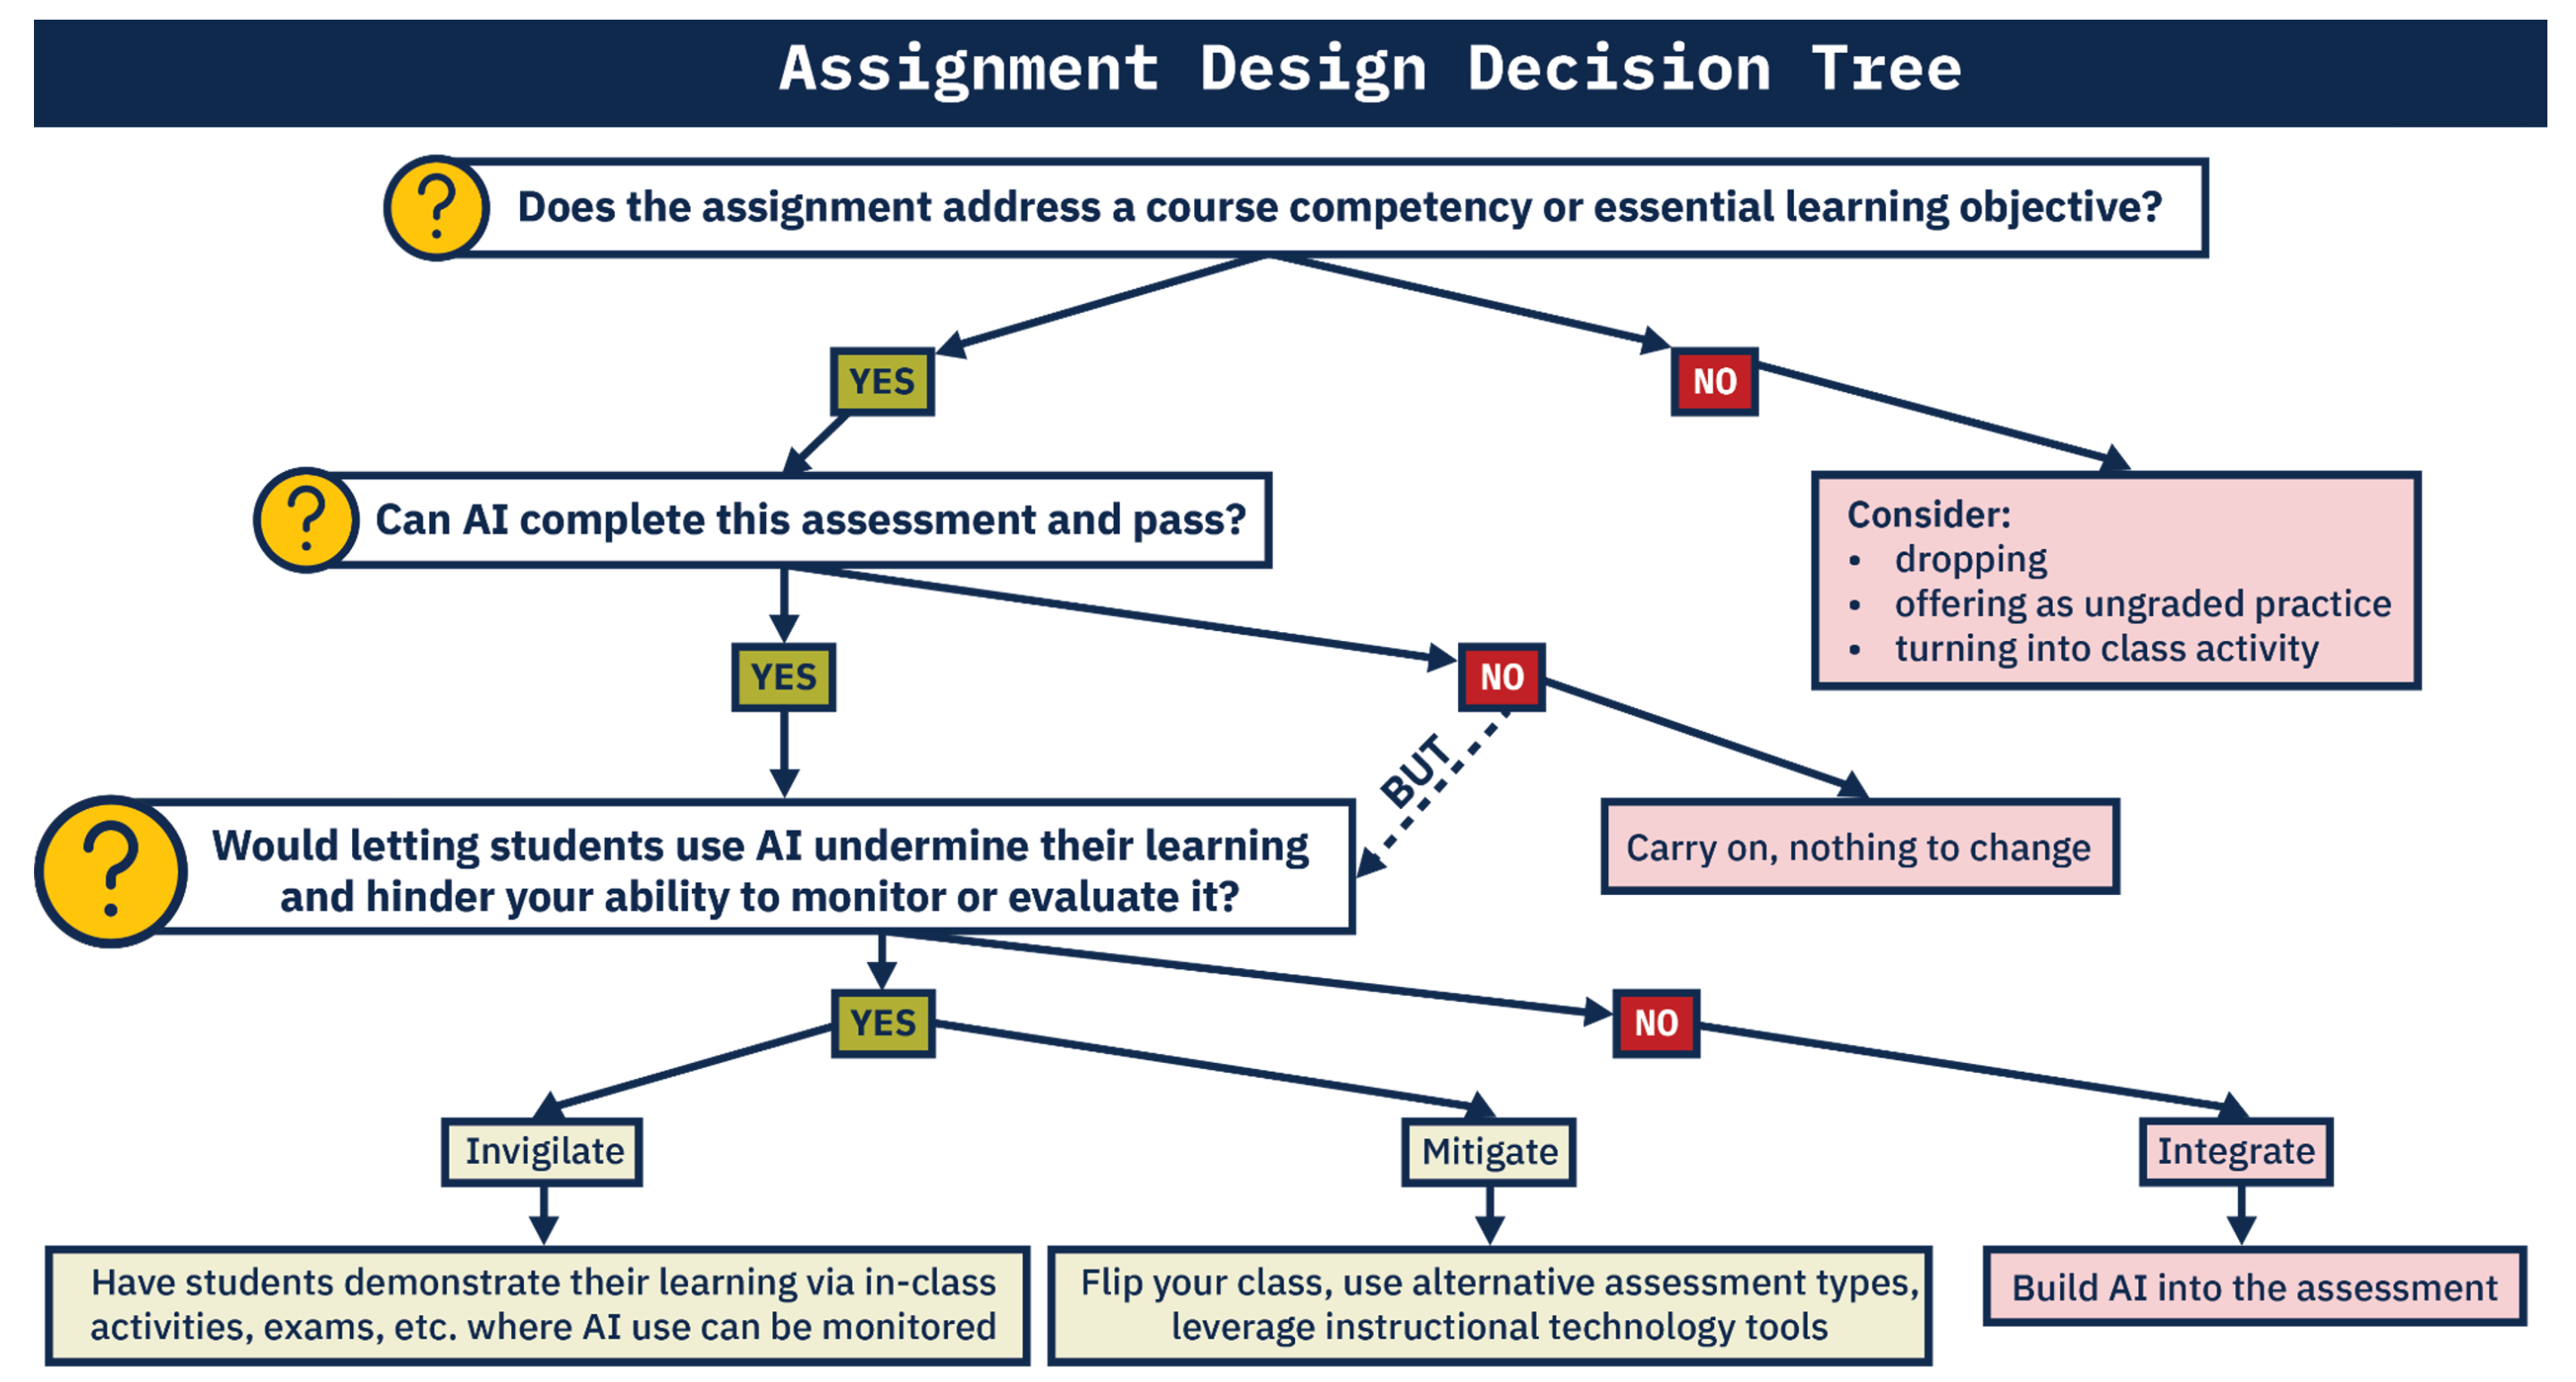
\includegraphics{dec_tree.png}

\hypertarget{considerations-for-writing-intensive-courses}{%
\paragraph*{Considerations for Writing-intensive Courses}\label{considerations-for-writing-intensive-courses}}
\addcontentsline{toc}{paragraph}{Considerations for Writing-intensive Courses}

For writing-intensive courses, the committee recognizes there are specific challenges to be addressed. Below is a summary of the guidance provided:

\begin{quote}
\begin{itemize}
\item
  GenAI will transform traditional academic writing, multimodal/multimedia composition, and creative expression in every U-M school and college.
\item
  It is imperative that instructors continue to teach writing as well as multimedia/multimodal composition.
\item
  GenAI presents opportunities and potential benefits. It can be used at any point in the writing process to complement and expand students' thinking, project planning, brainstorming, research, outlining, drafting, and revision processes. There are risks involved in using GenAI in these ways: use of GenAI may impair original thinking and problemsolving; students' privacy is not protected; the output may contain fabrications, falsifications, biases, or errors. Students are nonetheless responsible for the work they turn in, including the truthfulness, academic integrity, and biases of content.
\item
  GenAI tools can be used as a cheating machine, so threats to academic integrity should be anticipated and mitigated in U-M's academic misconduct policies and in syllabus statements.
\item
  Instead of eliminating writing assignments, instructors should consider how they might adapt their goals for writing assignments to new GenAI environments.
\end{itemize}
\end{quote}

\hypertarget{other-u-m-guidance}{%
\section{Other U-M Guidance}\label{other-u-m-guidance}}

Presently, the University of Michigan has the following:

\begin{itemize}
\item
  \href{https://safecomputing.umich.edu/protect-the-u/safely-use-sensitive-data/AI-and-UM-Data}{Artificial Intelligence and U-M Institutional Data - IT Guidance}

  \begin{itemize}
  \item
    Highlights:

    \begin{quote}
    \emph{``Accordingly, as with any other IT service or product with no university contract or agreement, AI tools should only be used with institutional data classified as LOW.~\href{https://safecomputing.umich.edu/protect-the-u/safely-use-sensitive-data/classification-levels}{See~U-M~Data Classification Levels for descriptions and examples of each data classification}.}

    \emph{Do not use ChatGPT or other AI with information such as student information regulated by FERPA, human subject research information, health information, HR records, etc.''}
    \end{quote}
  \end{itemize}
\item
  \href{https://guides.lib.umich.edu/c.php?g=1039501\&p=9763907}{GenAI section in U-M `Introduction to Academic Integrity'}
\end{itemize}

\hypertarget{ross}{%
\section{Ross}\label{ross}}

{[}PLACEHOLDER{]}

\hypertarget{community-perspective}{%
\section{Community Perspective}\label{community-perspective}}

\url{https://www.maisi.club/about}

\url{https://fordschool.umich.edu/news/2023/u-m-experts-we-need-emphasize-ais-societal-impacts-over-technological-advancements}

\hypertarget{publicly-available-generative-ai}{%
\chapter{Publicly Available Generative AI}\label{publicly-available-generative-ai}}

\hypertarget{text}{%
\section{Text}\label{text}}

\hypertarget{images}{%
\section{Images}\label{images}}

\hypertarget{music}{%
\section{Music}\label{music}}

\hypertarget{video}{%
\section{Video}\label{video}}

\hypertarget{speech-synthesis}{%
\section{Speech Synthesis}\label{speech-synthesis}}

\hypertarget{organizational-challenges}{%
\chapter{Organizational Challenges}\label{organizational-challenges}}

\hypertarget{current-responses}{%
\section{Current Responses}\label{current-responses}}

\hypertarget{future-plans}{%
\section{Future Plans}\label{future-plans}}

\hypertarget{individual-challenges}{%
\chapter{Individual Challenges}\label{individual-challenges}}

\hypertarget{current-responses-1}{%
\section{Current Responses}\label{current-responses-1}}

\hypertarget{future-plans-1}{%
\section{Future Plans}\label{future-plans-1}}

\hypertarget{final-thoughts}{%
\chapter{Final Thoughts}\label{final-thoughts}}

\hypertarget{works-cited}{%
\chapter{Works Cited}\label{works-cited}}

\end{document}
